% !TEX encoding = UTF-8
% !TEX TS-program = pdflatex
% !TEX root = ../tesi.tex

%**************************************************************
\chapter{Analisi dei requisiti}
\label{cap:analisi-requisiti}
%**************************************************************

\intro{Breve introduzione al capitolo}\\


\section{Casi d'uso}

In questa sezione vengono trattati i casi d'uso riguardanti l'interazione dell'utente con l'interfaccia visiva dell'applicativo. Con i casi d'uso si vuole mostrare una panoramica delle funzionalità dell'applicativo. Vengono inseriti gli Use Cases DiagramG e la loro descrizione secondo le specifiche UML2.0G. L’attore principale è sempre l'utente generico autenticato oppure l'utente  amministrativo autenticato. \\
 Pagina iniziale 
\begin{figure}[!h] 
    \centering 
    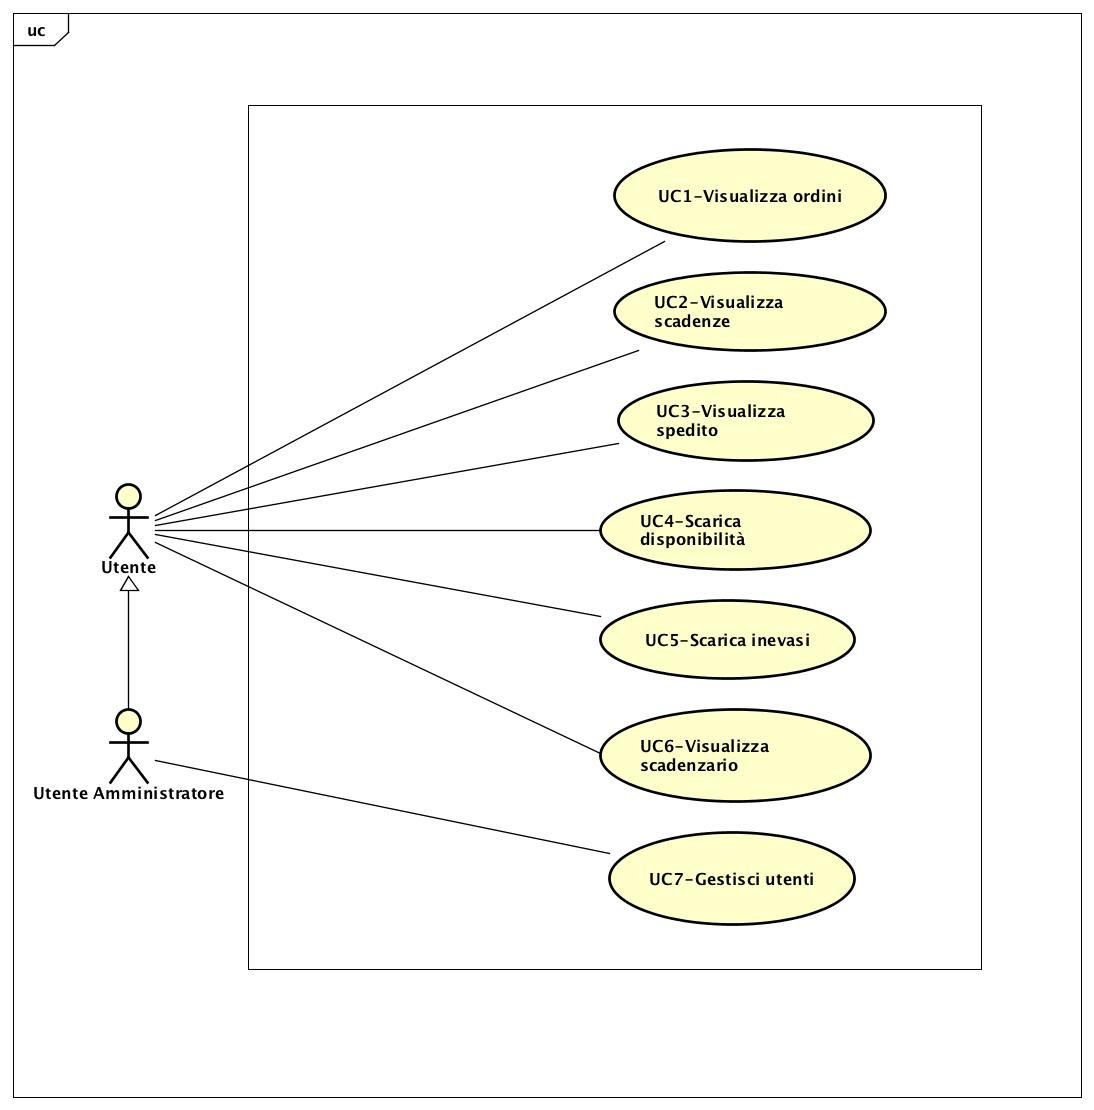
\includegraphics[width=1.0\columnwidth]{usecase/UseCase_Diagram0} 
    \caption{Use Case - UC0: Scenario principale}
\end{figure} 
\textbf{Attori primari:}   Utente autenticato\\

\textbf{Descrizione:} L’utente generico può visualizzare la lista degli ordini, può visualizzare le scadenze, lo spedito, la disponibilità degli ordini, gli inevasi e lo scadenzario. L’utente amministratore (che è una generalizzazione dell’utente generico) può gestire gli utenti, attivando una licenza, rimuovere gli utenti, associare un utente con un’account B2B e rimuovere un’associazione. \\

\textbf{Precondizione:}  Il sistema funziona correttamente e visualizza la pagina principale correttamente. \\

\textbf{Postcondizione:} Il sistema ha ricevuto uno dei comandi eseguiti dall’utente ed è stato scaricato il file che visualizza le informazioni richieste dall’utente oppure è stato aperta la pagina dell’amministrazione degli utenti nel caso dell’utente amministratore.\\


\textbf{Flusso base degli eventi:}   
\begin{itemize}


\item L’attore visualizza la lista del tipo di ordine da selezionare (UC1);
\item L’attore può visualizzare la lista del tipo di scadenze da selezionare (UC2);
\item L’attore può visualizzare la lista del tipo di spedito da selezionare (UC3);
\item L’attore può scaricare il documento aggiornato  del report di Disponibilità (UC4);
\item L’attore può scaricare il documento aggiornato del report Inevaso (UC5);
\item L’attore può visualizzare la lista del tipo di scadenzario da selezionare (UC6);
\item L’attore (utente amministratore) può visualizzare la lista dei comandi per gestire l’associazione tra utenti, l’eliminazione e la gestione delle licenze (UC7);

\end{itemize}



Amministrazioni utenti \\\\

\begin{figure}[!h] 
    \centering 
    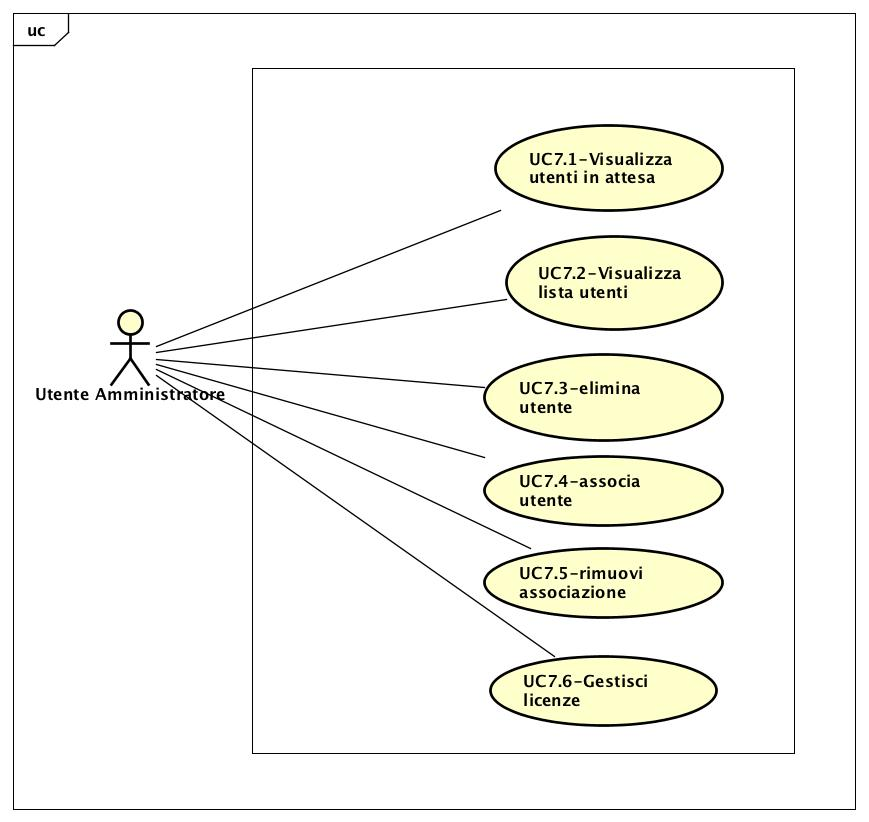
\includegraphics[width=1.0\columnwidth]{usecase/UseCase_Diagram1} 
    \caption{Use Case - UC0: Scenario principale}
\end{figure} 

\textbf{Attori primari:}   Utente amministratore autenticato\\


\textbf{Descrizione:} L’utente amministratore può visualizzare la lista degli utenti che risultano attivi con una licenza, visualizzare gli utenti che sono in attesa ad essere registrati nel sistema (cioè gli utenti che hanno fatto richiesta per essere registrati con una licenza ma che non sono ancora accettati da un amministratore). L’utente amministratore può eliminare un utente generico può gestire la licenza, inserendo una nuova oppure visualizzare lo stato di quelle attive. Infine l’utente amministratore può effettuare un’associazione tra l’utente B2B ed il suo account telegram oppure può eliminare un’associazione precedentemente creata. \\

\textbf{Precondizione:}   Il sistema funziona correttamente e visualizza la pagina all’amministrazione utenti correttamente. \\

\textbf{Postcondizione:}  L’utente amministratore è stato in grado ad effettuare correttamente  un’operazione da lui voluta nella pagina di gestione utenti.\\


\textbf{Flusso base degli eventi:} 

\begin{itemize}

\item L’utente amministratore visualizza la lista degli utenti in attesa ad essere registrati (UC7.1);
\item L’utente amministrativo visualizza la lista degli utenti registrati correttamente con una licenza valida (UC7.2);
\item L’utente amministrativo elimina un utente rimuovendo anche la relativa licenza (UC7.3);
\item L’utente amministrativo associa un utente B2B con il suo account telegram (UC7.4);
\item L’utente amministrativo rimuove l’associazione di un utente B2B con l’account telegram (UC7.5);
\item L’utente visualizza la lista dei comandi per l’amministrazione di un utente generico (UC7.6);


\end{itemize}  



Ordini del giorni \\\\

\begin{figure}[!h] 
    \centering 
    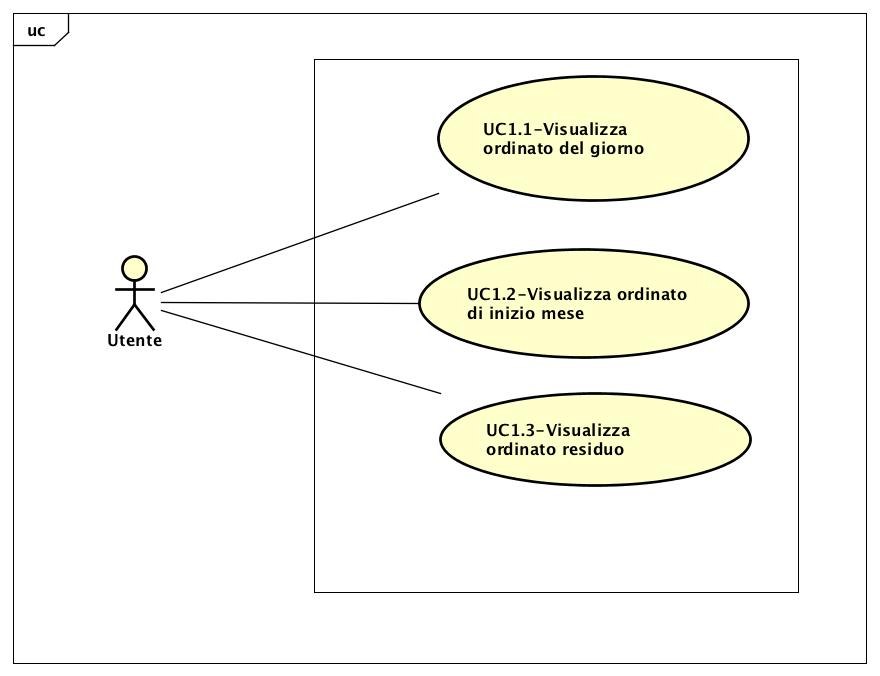
\includegraphics[width=1.0\columnwidth]{usecase/UseCase_Diagram2} 
    \caption{Use Case - UC0: Scenario principale}
\end{figure} 

\textbf{Attori primari:} Utente generico ed utente amministratore autenticati
\\


\textbf{Descrizione:} L’utente (generico oppure amministratore) può scegliere di visualizzare il report “ordinato del giorno”, “ordinato di inizio mese” o “ordinato residuo”. \\

\textbf{Precondizione:} Il sistema funziona correttamente e visualizza la pagina per poter scaricare gli ordinati correttamente. \\

\textbf{Postcondizione:}  L’utente generico oppure amministratore è stato in grado di visualizzare correttamente  un “ordinato” da lui voluto nella pagina di visualizzazione ordini. \\


\textbf{Flusso base degli eventi:} 

\begin{itemize}

\item L’utente visualizza i valori inerente all’ordinato del giorno (UC1.1);
\item L’utente visualizza i valori inerente all’ordinato di inizio mese (UC1.2);
\item L’utente visualizza i valori inerente all’ordinato residuo (UC1.3);

\end{itemize}



Scadenze \\\\

\begin{figure}[!h] 
    \centering 
    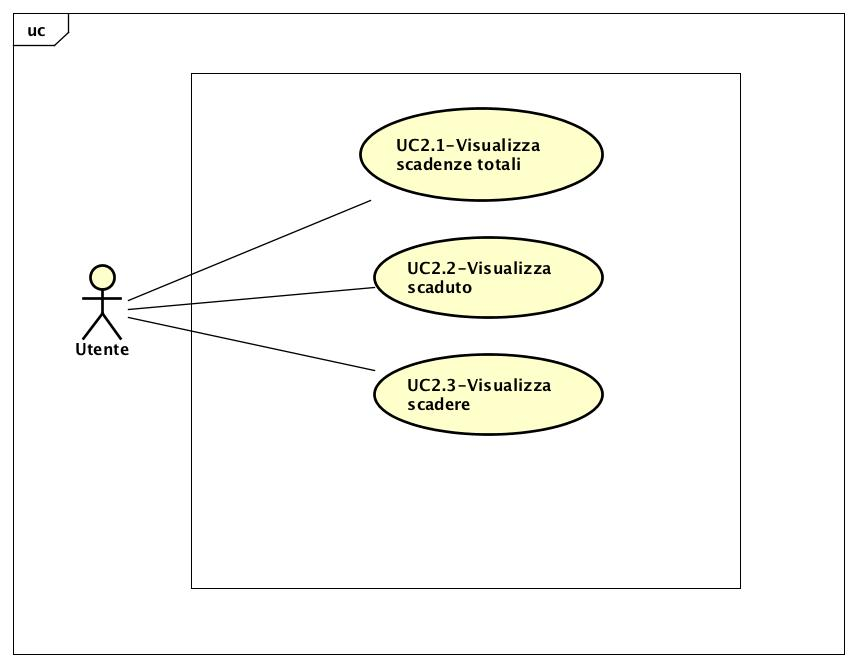
\includegraphics[width=1.0\columnwidth]{usecase/UseCase_Diagram3} 
    \caption{Use Case - UC0: Scenario principale}
\end{figure} 


\textbf{Attori primari:} Utente generico ed utente amministratore autenticati
\\


\textbf{Descrizione:}  L’utente (generico oppure amministratore) può scegliere di visualizzare l’ammontare delle “scadenze totali”, dello “scaduto” oppure “scadere”.  \\

\textbf{Precondizione:} Il sistema funziona correttamente e visualizza la pagina per poter visualizzare le scadenze correttamente. \\

\textbf{Postcondizione:} L’utente generico oppure amministratore è stato in grado di visualizzare correttamente le scadenze da lui volute nella pagina di visualizzazione scadenze. \\


\textbf{Flusso base degli eventi:} 

\begin{itemize}

\item L’utente visualizza i valori inerenti alle scadenze totali (UC2.1);
\item L’utente visualizza i valori inerenti allo scaduto (UC2.2);
\item L’utente visualizza i valori inerenti allo scadere (UC2.3);


\end{itemize}




Gli spediti \\\\

\begin{figure}[!h] 
    \centering 
    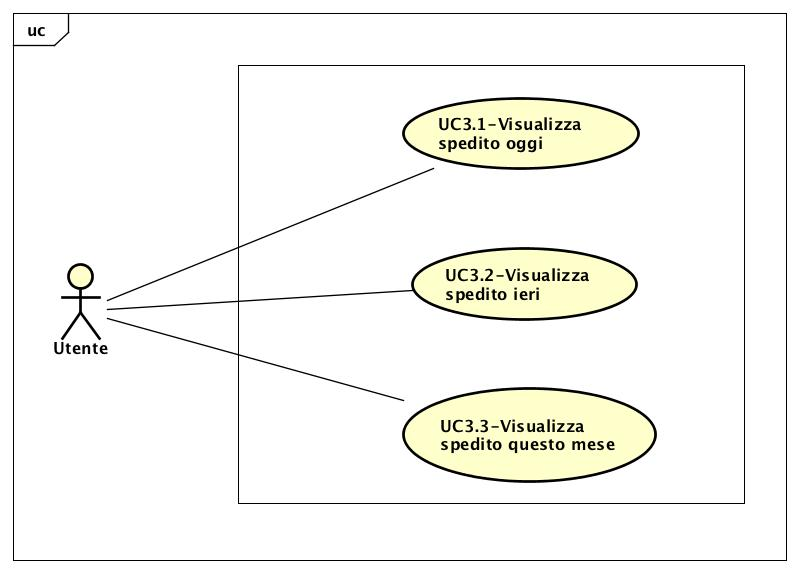
\includegraphics[width=1.0\columnwidth]{usecase/UseCase_Diagram4} 
    \caption{Use Case - UC0: Scenario principale}
\end{figure} 

\textbf{Attori primari:} Utente generico ed utente amministratore autenticati
\\


\textbf{Descrizione:}  L’utente (generico oppure amministratore) può scegliere di visualizzare l’ammontare dello “spedito oggi”, dello “spedito ieri” oppure “spedito questo mese”.  \\

\textbf{Precondizione:} Il sistema funziona correttamente e visualizza la pagina per poter visualizzare gli spediti correttamente. \\

\textbf{Postcondizione:} L’utente generico oppure amministratore è stato in grado di visualizzare correttamente gli spediti da lui volute nella pagina di visualizzazione scadenze.  \\


\textbf{Flusso base degli eventi:} 

\begin{itemize}

\item L’utente visualizza i valori inerenti allo spedito oggi (UC3.1);
\item L’utente visualizza i valori inerenti allo spedito ieri (UC3.2);
\item L’utente visualizza i valori inerenti allo spedito questo mese (UC3.3);

\end{itemize}


Scadenzario \\\\

\begin{figure}[!h] 
    \centering 
    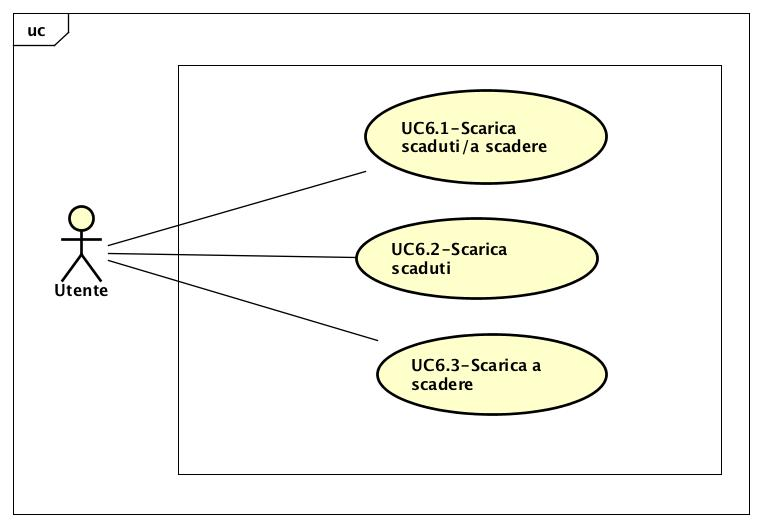
\includegraphics[width=1.0\columnwidth]{usecase/UseCase_Diagram5} 
    \caption{Use Case - UC0: Scenario principale}
\end{figure} 

\textbf{Attori primari:} Utente generico ed utente amministratore autenticati
\\


\textbf{Descrizione:}   L’utente (generico oppure amministratore) può scegliere di scaricare il documento che rappresenta il report di “scaduti/a scadere”, “scaduti” oppure “a scadere”.   \\

\textbf{Precondizione:}  Il sistema funziona correttamente e visualizza la pagina per poter scaricare lo scadenzario correttamente. \\

\textbf{Postcondizione:} L’utente generico oppure amministratore è stato in grado di scaricare correttamente lo scadenzario da lui volute nella pagina di visualizzazione scadenzario.  \\


\textbf{Flusso base degli eventi:} 

\begin{itemize}

\item L’utente scarica il report inerente agli scaduti/a scadere (UC6.1);
\item L’utente scarica il report inerente agli scaduti  (UC6.2);
\item L’utente scarica il report inerente allo scadere (UC6.3);


\end{itemize}


\begin{tabular}{ |p{2cm}|p{8cm}|p{2cm}| }
 

 \hline
\textbf{ Requisito}   &  \textbf{Descrizione}    &  \textbf{    Use Case} \\ 

 \hline
  RF-0 &   L’attore può visualizzare la pagina principale per poter scegliere uno delle funzionalità presenti   & UC0 \\
 \hline
RF-1 &   L’attore visualizza la lista del tipo di ordine da selezionare (l’ammontare degli ordini in euro)  & UC1 \\
 \hline
 RF-2 & L’attore può visualizzare l’ordinato del giorno & UC1.1 \\
\hline
RF-3 & L’attore può visualizzare l’ordinato di inizio mese & UC1.2 \\
\hline
RF-4  &  L’attore può visualizzare l’ordinato residuo  & UC1.3 \\
\hline  
RF-5  & L’attore visualizza la lista del tipo di scadenze da selezionare  (l’ammontare delle scadenze in euro)  & UC2 \\
\hline
RF-6   & L’attore può visualizzare le scadenze totali   & UC2.1 \\
\hline
RF-7  &  L’attore può visualizzare lo scaduto & UC2.2 \\
\hline
RF-8   &  L’attore può visualizzare lo scadere & UC2.3 \\
\hline
RF-9   &  L’attore visualizza la lista del tipo di spedito da selezionare  (l’ammontare dello spedito in euro) & UC3 \\
 \hline
 RF-10   &  L’attore può visualizzare lo spedito di oggi & UC3.1 \\
  \hline
  RF-11   &  L’attore può visualizzare lo spedito di ieri & UC3.2 \\
   \hline
   RF-12  & L’attore può visualizzare lo spedito del mese  & UC3.3 \\
   \hline
   RF-13  &  L’attore può scaricare il documento aggiornato del report di Disponibilità & UC4 \\
   \hline
   RF-14  & L’attore può scaricare il documento aggiornato del report Inevaso   & UC6 \\
   \hline
RF-15    &  L’attore può visualizzare la lista dei comandi per gestire l’associazione tra utenti, l’eliminazione e la gestione delle licenze & UC7 \\
 \hline
   RF-16     & L’attore può visualizzare gli utenti in attesa di registrazione   & UC7.1 \\
\hline
RF-17   & L’attore può visualizzare la lista gli utenti già registrati   & UC7.2 \\
\hline
RF-18   & L’attore può eliminare un utente  & UC7.3 \\
\hline
RF-19   &  L’attore può associare un utente B2B con il suo account telegram  & UC7.4 \\
\hline
RF-20  &  L’attore può rimuovere l’associazione di un utente B2B con il suo account telegram & UC7.5 \\
\hline
RF-21   &  L’attore può gestire la licenza di un utente  & UC7.6 \\
\hline
RF-22   &  L’attore può visualizzare le licenze degli utenti & UC7.7 \\
\hline
RF-23   & L’attore può inserire una  licenza  & UC7.8 \\
\hline
\end{tabular}
\\ \\ \\ \\

Tabella con requisiti qualitativi \\

\begin{tabular}{ |p{2cm}|p{8cm}|p{2cm}| }
 

 \hline
\textbf{ Requisito}   &  \textbf{Descrizione}    &  \textbf{    Use Case} \\ 
\hline
RQ-1  &  Il codice sviluppato deve essere versionato con il sistema RTC integrato nello strumento Eclipse & Azienda \\
\hline
RQ-2 &  Si deve usare il software Kettle per la gestione ETL & Azienda \\
\hline
\end{tabular}
\\ \\ \\ \\

Tabella con i vincoli \\



\begin{tabular}{ |p{2cm}|p{8cm}|p{2cm}| }
 

 \hline
\textbf{ Requisito}   &  \textbf{Descrizione}    &  \textbf{    Use Case} \\ 
\hline

RV-1 &  Il prodotto deve essere sviluppato secondo rispettando  gli standard ISO aziendali & Azienda \\
\hline
RV-2 &  L’interfaccia front-end deve essere sviluppata, basandosi sulla piattaforma telegram per sfruttare le notifiche push  & Azienda \\
\hline
RV-3 &  La logica di BI deve essere sviluppata come web-services sul server Java Tomcat& Azienda \\
\hline
RV-4 & Come DBMS si deve usare PostgresSQL & Azienda \\
\hline
\end{tabular}











